\chapter{\IfLanguageName{dutch}{Praktische performantie}{Practical performance}}
\label{ch:praktischePerformantie}

%=======================================================================
% Technische perfromantie hoofdstuk
%=======================================================================

React biedt talloze oplossing voor het bevorderen van performantie, om een kijk te krijgen op enkele van de meest courante technieken wordt er in dit hoofdstuk een overzicht opgesteld. Enkele van de oplossingen die worden aangehaald zijn nagebootst binnen een testomgeving, waarna de resultaten worden geanalyseerd. Neem op voorhand aan dat dit niet de enige mogelijkheden zijn voor het optimaliseren van performantie. De voorgestelde technieken zijn onderverdeeld in 3 categorieën: \\

\begin{itemize}[label={}]
    \item \textbf{Native}:
    De oplossingen die React ons zelf bied als zijnde deel van de core functionaliteiten \newline
    \item \textbf{Framework}:
    Mogelijkheden die we specifiek kunnen toepassen door het gebruik van React  \newline
    \item \textbf{Tools}:
    Functionaliteiten afkomstig van een derde partij die we kunnen integreren in de codebase
\end{itemize}

\section{\IfLanguageName{dutch}{Native}{Native}}
\label{sec:nativeOplossingen}

Door React in scope te plaatsen is er toegang tot de React top-level \gls{api}. Zoals wordt aangegeven in figuur~\ref{fig:reactImport} op pagina~\pageref{fig:reactImport} is de import het aanspreekpunt voor de \gls{api} en maakt alle React functionaliteiten aanspreekbaar. Zoals wordt aangegeven in figuur~\ref{fig:reactImport} op pagina~\pageref{fig:reactImport}.

\begin{figure}[H]
    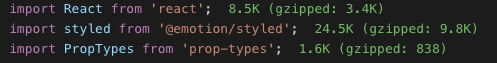
\includegraphics[width=\linewidth]{ReactInScope.png}
    \caption{React in scope}
    \label{fig:reactImport}
\end{figure}

\subsection{\IfLanguageName{dutch}{Gebruiken van de Fragment tag}{Usage of the Fragment tag}}
\label{sec:fragmentsPraktisch}

Een probleem dat vaak voorkomt wanneer het gaat om performantie is het lezen en schrijven naar het \gls{dom}. \gls{dom} manipulaties zijn op zich zeer belastend en vragen veel \gls{cpu}-tijd. Als het \gls{dom} vol wordt gestoken met nestingen van nodes ontstaat er vanzelfsprekend vertraging.\\
In sectie~\ref{sec:fragments} op pagina~\pageref{sec:fragments} werd uitgelegd hoe React fragments het \gls{dom} vrijhouden van een overrompeling aan nutteloze tags, waaronder vooral <div> tags.

\subsection{\IfLanguageName{dutch}{Extenden van React.PureComponent}{Extend of React.PureComponent}}
\label{sec:pureComponent}

Pure component is exact hetzelfde als een gewoon component in React. Het verschil tussen beiden ligt bij het aanroepen van de lifecycle methode shouldComponentUpdate(), die op een andere manier uitgevoerd wordt. Bij een normaal component zal er altijd een re-render uitgevoerd worden wanneer er iets aan props of state veranderd. In een pure component wordt er in de shouldComponentUpdate functie aan shallow comparison gedaan van props en state.\\
Bij shallow comparison worden de waarden en referenties van de vorige props en state vergeleken met de volgende. Deze controle is goedkoop, zeker in vergelijking met het telkens re-renderen van een component. Het nadeel is dat er geen controle wordt gedaan voor de waarden in geneste objecten. \\
Het omzetten gaat ervoor zorgen dat er minder re-renders gebeuren. Dit wordt ook overgedragen naar de kinderen van een pure component, daardoor is het af te raden voor componenten met kinderen, tenzij al deze ook pure components worden.\\
Het is een best practice om een gewoon klasse component om te zetten wanneer het eenvoudige state en props bevat. Het gebruik van een pure component geeft een performantie boost zonder dat er veel aanpassingen moeten worden gedaan aan de initiële code.\\
Figuur~\ref{fig:extendPureComponent} op pagina~\pageref{fig:extendPureComponent} geeft aan waar de aanpassing plaats vindt.

\begin{figure}[H]
    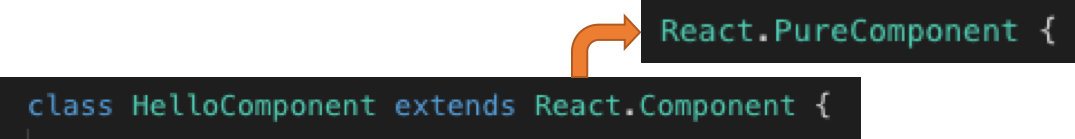
\includegraphics[width=\linewidth]{ExtendPureComponent.png}
    \caption{Veranderen van component naar pure component}
    \label{fig:extendPureComponent}
\end{figure}

%\subsubsection{\IfLanguageName{dutch}{Experiment}{Experiment}}
%\label{sec:pureComponentExp}


\subsection{\IfLanguageName{dutch}{Wikkelen in React.Memo}{Wrap in React.Memo}}
\label{sec:memo}

Memoization is een techniek voor het optimaliseren van snelheid in computer programma's. Door de dure functies, die regelmatig worden uitgevoerd, op te slaan in het cache geheugen kunnen ze veel sneller uitgevoerd worden in de toekomst. React memo werkt volgens hetzelfde principe.\\
React Memo is gelijkaardig aan het extenden van een pure component, het geeft controle over het renderen van functionele componenten. Als een functioneel component wordt gewikkeld in React.memo() worden bij elke re-render enkel de \gls{ui}-elementen opnieuw gerenderd die geüpdatet props nodig hebben.

\subsection{\IfLanguageName{dutch}{React lazy}{React lazy}}
\label{sec:lazy}

Het integreren van code-splitting helpt voor het lazy loaden van componenten. Alles tegelijk in één keer downloaden voor het inladen van de pagina is niet optimaal. \gls{ui} elementen worden ingeladen zonder dat er ooit interactie is met de gebruiker. Tijdens lazy loading wordt gewacht om code in te laden tot wanneer het wel degelijk nodig is.\\
Figuur~\ref{fig:lazyLoading} op pagina~\pageref{fig:lazyLoading} toont een voorbeeld voor het lazy loaden van een component.

\begin{lstlisting}[caption=Lazy loading a component, label={fig:lazyLoading}]
    // MyComponent.js
    class MyComponent extends Component{
        render() {
            return (<div>MyComponent</div>);
        }
    }
    
    // App.js
    import React from 'react';
    
    const MyComponent = React.lazy(()=>import('./MyComponent.js'))
        function AppComponent() {
            return (
                <div>
                    <MyComponent />
                </div>
            );
    }
\end{lstlisting}

\subsubsection{\IfLanguageName{dutch}{Suspense}{Suspense}}
\label{sec:suspens}

Suspense is een concept dat werd geïntroduceerd met de komst van React lazy in React versie 16.6. Het bied een fallback functie voor componenten die lazy loaded zijn. Tijdens het dynamisch inladen van een component kan er een laad tijd ontstaan afhankelijk van de document grootte. Figuur~\ref{fig:suspenseLazy} op pagina~\pageref{fig:suspenseLazy} geeft aan hoe die laadtijd wordt opgevangen met suspense.\\

\newpage
\begin{lstlisting}[caption=Lazy loading met suspense, label={fig:suspenseLazy}]
    // MyComponent.js
    class MyComponent extends Component{
        render() {
            return (<div>MyComponent</div>);
        }
    }
    
    // App.js
    import React, { Suspense } from 'react';
    
    const MyComponent = React.lazy(()=> import('./MyComponent.js'));
    function AppComponent() {
        return (
            <Suspense fallback={<div>Loading ...</div>} >
                <MyComponent />
            </Suspense>
        );
    }
\end{lstlisting}

\section{\IfLanguageName{dutch}{Framework}{Framework}}
\label{sec:frameworkOplossingen}

\subsection{\IfLanguageName{dutch}{Propagatie}{Propagation}}
\label{sec:propagatie}

Bij propagatie geven we properties mee aan een component, om het een bepaalde vorm te geven aan het deel van de \gls{ui} die geretourneerd wordt. In praktijk is het mogelijk om alle props die een ouder bezit door te geven aan zijn kinderen door alle props te spreaden in de component tag. Sectie~\ref{sec:spreadOperator} op pagina~\pageref{sec:spreadOperator} geeft aan hoe de spread operator functioneert en hoe props worden gespread in een component.\\
Het spreaden van het volledige prop object in de component tag is niet altijd een best practice. Wanneer het props object exact de gewenste waarden bevat om door te geven aan een volgend component is er geen probleem. Als er geen zekerheid is over de inhoud van het props object is het een bad practice om deze te spreaden. Door het doorsturen van een inhoudelijk onbekend props object is er grote kans dat we het \gls{dom} vervuilen door properties zonder afhankelijkheid toe te kennen aan componenten.

\subsection{\IfLanguageName{dutch}{Function calls in de render functie}{Function calls in the render function}}
\label{sec:functionCalls}

Figuur~\ref{fig:funcCalls} op pagina~\pageref{fig:funcCalls} toont twee voorbeelden voor het uitvoeren van een functie binnen in de render functie van een component. Het eerste voorbeeld zal telkens een nieuwe referentie aanmaken voor de functie wanneer hij opnieuw gerenderd wordt. Constant nieuwe referenties aanmaken is een bad practice in het performance handboek.\\
Voor het tegengaan van het steeds opnieuw aanmaken van een referentie maken we een arrow functie aan buiten de render. Wanneer de functie nu wordt aangeroepen wordt de referentie naar de arrow functie bewaard.

\newpage
\begin{lstlisting}[caption=Lazy loading met suspense, label={fig:funcCalls}]
     // Functie uitvoeren in de render fucntie
     class MyComponent extends React.Component {
        render() {
            return (
                <button onClick={() => { console.log('Hey, you clicked!'); }}>Click me!</button>
            );
        }
    }
    
    // Functie uitvoeren buiten de render functie
    class MyComponent extends React.Component {
        const handleClick = () => {
            console.log('Hey, you clicked!');
        }
        
        render() {
            return (
                <button onClick={this.handleClick}>Click me!</button>
            );
        }
    }
\end{lstlisting}

            
